\section{Algorithms}\label{sec:algorithms}
This chapter describes how scalafmt formats Scala code.
We will see that scalafmt's design is inspired by ClangFormat and dartfmt.
However, we believe our design makes a valuable contribution in that it leverages functional programming principles to maximise code reuse and extensibility.

\subsection{Design}
Figure~\ref{fig:architecture} shows a broad architectural overview of scalafmt.
\begin{figure}
  \centering
  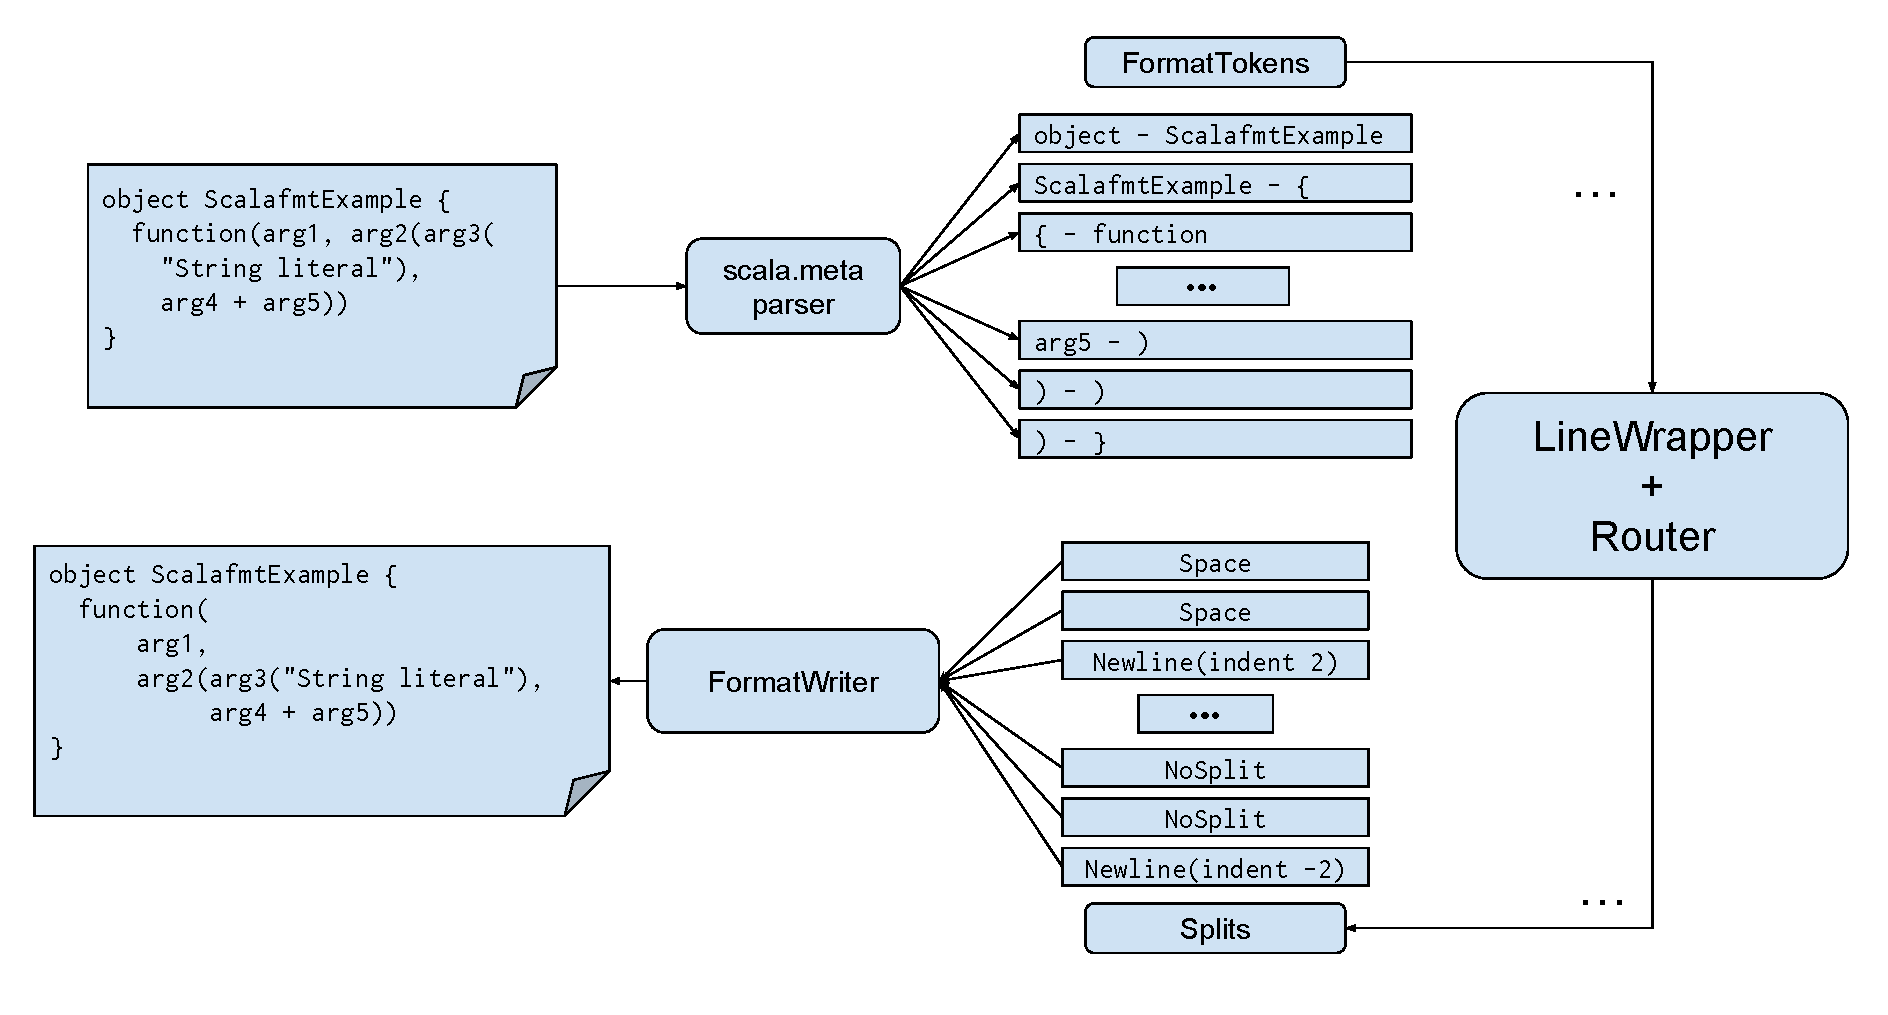
\includegraphics[width=\textwidth]{img/architechture.pdf}
  \caption{Scalafmt architecture}
  \label{fig:architecture}
\end{figure}
First, scalafmt parses a source file using scala.meta.
Next, we feed a sequence of \emph{FormatToken} data types into a \emph{LineWrapper}.
The LineWrapper uses a \emph{Router} to construct a weighted directed graph and run a best-first search to find an optimal formatting layout for the whole file.
Finally, the LineWrapper feeds a sequence of \emph{Split} data types into the \emph{FormatWriter}, which constructs a new reformatted source file.
The following sections explain these data types and abstractions in detail.

\subsection{Data structures}
Scalafmt leverages a few carefully designed data structure to allow an implementation that emphasizes correctness and maintainability.

\subsubsection{FormatToken}
A \emph{FormatToken} is a pair of two non-whitespace tokens.
Listing~\ref{lst:format_token} shows the definition of the FormatToken data type.
\lstinputlisting[label={lst:format_token}, caption=FormatToken definition]{code/format_token.scala}
As shown in the architecture overview in figure~\ref{fig:architecture}, each token except the beginning and end of file tokens appear twice in the sequence of FormatTokens: once as the \texttt{left} member and once as the \texttt{right} member.
In a nutshell, the job of the LineWrapper is to convert each FormatToken into a \emph{Split}

\subsubsection{Decision}\label{sec:decision}
A Decision is a pair of a FormatToken and a sequence of Splits.
Listing~\ref{lst:decision} shows the Definition of decision.
\lstinputlisting[label={lst:decision}, caption=Decision definition]{code/decision.scala}
The \emph{splits} member represents the possible splits that we can take at \emph{formatToken}.

\subsubsection{Policy}\label{sec:policy}
A \emph{Policy} is an enforced formatting layout over a region.
Listing~\ref{lst:policy} shows the definition of Policy.
\begin{minipage}{\linewidth}
  \lstinputlisting[label={lst:policy}, caption=Policy definition]{code/policy.scala}
\end{minipage}
A Policy is a partial function that should be applied to future Decisions up until the \emph{expire} token.
Policies easily compose using the Scala standard library \texttt{orElse} and \texttt{andThen} methods on PartialFunction\footnote{
  Careful eyes will observe that Policy is in fact a monoid with the empty partial function as identity and function composition as associative operator.}.
This enables a high-level way to express arbitrary formatting layouts over a region of code.

\subsubsection{Indent}\label{sec:indent}
An \emph{Indent} describes indentation over a region of code.
\lstinputlisting[label={lst:indent}, caption=Indent definition]{code/indent.scala}
Listing~\ref{lst:indent} shows the definition of Indent along with the algebraic data type \emph{Length}.
Length can either be \texttt{Num(n)} where $n$ represents an explicit number of spaces to indent by or \texttt{StateColumn} which is a placeholder the number of spaces required to vertically align by the current column.
Indent is type parameterized by Length so that, at some point, we can replace StateColumn placeholders with Nums to obtain a concrete number.
For example, given a scala.meta tree \texttt{expr}, the definition \texttt{Indent(Num(2), expr.tokens.last, inclusive=true)}
increases the indentation level by 2 spaces up to and including the last token of \texttt{expr}.
The \texttt{inclusive} member is set to false when the indentation should expire before the expire token, for example in a block wrapped by curly braces, since the closing curly brace should not be indented by 2 spaces.
The StateColumn placeholder is required to allow memoization of Splits, which is critical for performance reason as explained in section~\ref{sec:router} on the \emph{Router}.

\subsubsection{Split}
A \emph{Split} represents a (possibly empty) whitespace character to be inserted between two non-whitespace tokens.
Listing~\ref{lst:split} shows the rather intricate definition of the Split data type\footnote{
  For clarity reasons, a few less important members have been removed from the actual Split definition.}.
\begin{minipage}{\linewidth}
  \lstinputlisting[label={lst:split}, caption=Split definition]{code/split.scala}
\end{minipage}
The Split data type went through several generations of design before reaching its current structure.
Each member serves an important role.
The most important member of the Split type is the \emph{modification}.
A modification must be one of \texttt{NoSplit}, \texttt{Space} and \texttt{Newline}.
The \emph{cost} member represents the penalty for choosing this split.
The \emph{optimalToken} member enables an optimization explained in section~\ref{sec:optimal}.
The \emph{indents} member contains the indentation layers that this splits adds.
The \emph{line} member allows a powerful debugging technique explained in section~\ref{sec:router}.
The \emph{policy} and \emph{indents} members are explained in sections~\ref{sec:policy} and~\ref{sec:indent}, respectively.

\subsection{LineWrapper}
The LineWrapper is responsible for turning FormatTokens into Splits.
To accomplish this, the LineWrapper employs a \emph{Router} and abest-first search.

\subsubsection{Router}\label{sec:router}
The Router's role is to produce a Decision given a FormatToken.
Figure~\ref{fig:router} shows all possible formatting layout for the small input \texttt{val x = y + z}.
\begin{figure}
  \centering
  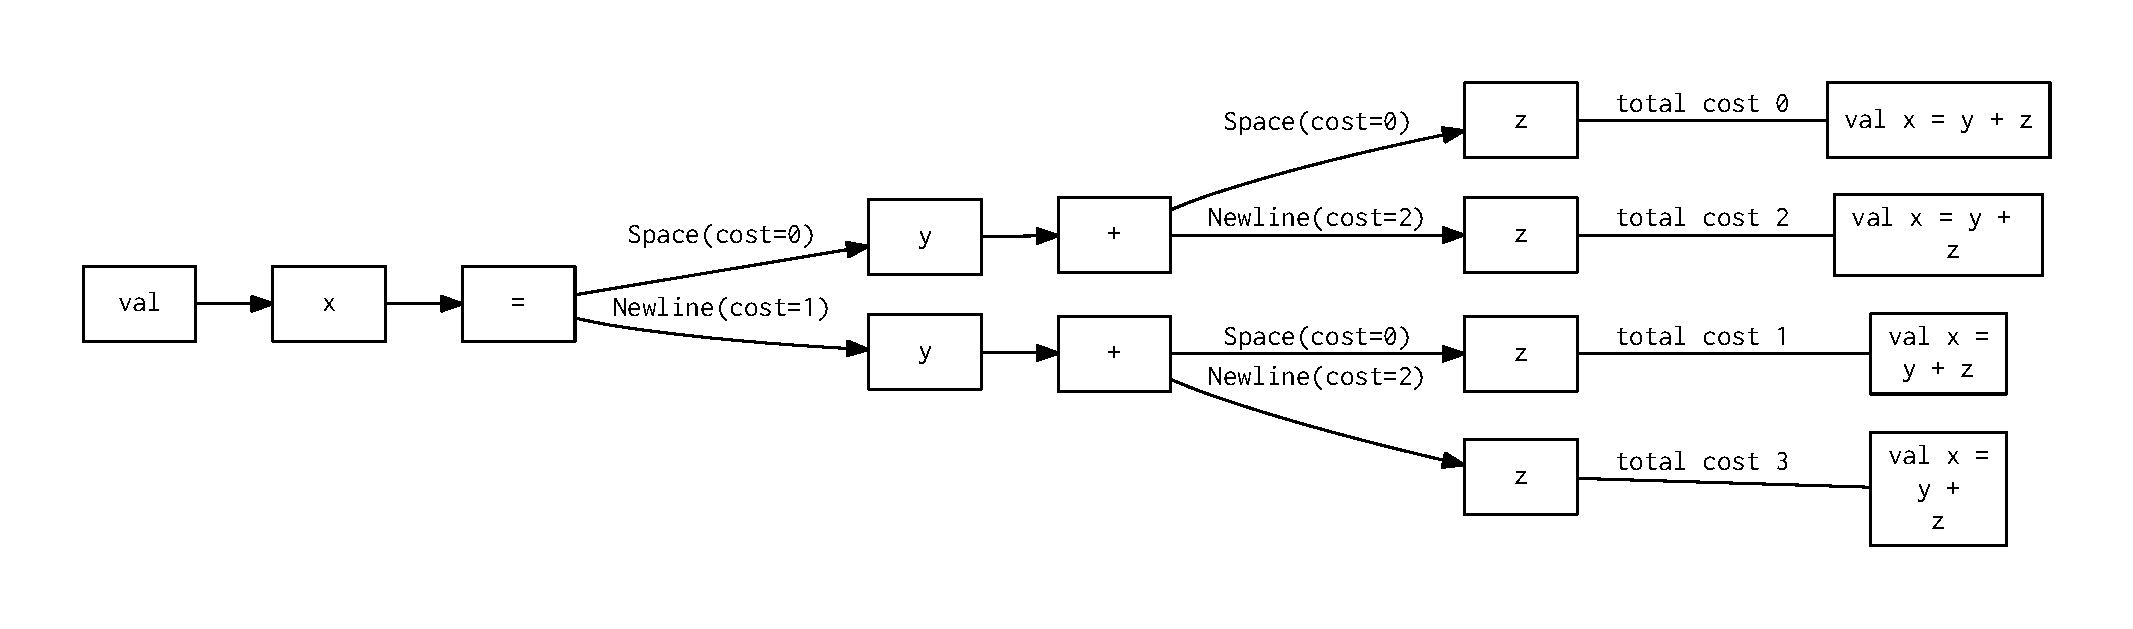
\includegraphics[width=\textwidth]{target/router.pdf}
  \caption{Example graph produced by Router}
  \label{fig:router}
\end{figure}
The Router must in this case figure out the correct combination of modifications and costs to associate with each FormatToken.
This is no easy task since a FormatToken can be any pair of two tokens.
How do we go about implementing a Router?

The Router is implemented as one single large pattern match on a FormatToken.
Listing~\ref{lst:match} shows how to pattern match on a FormatToken.
\lstinputlisting[label={lst:match}, caption=Pattern matching on FormatToken]{code/match.scala}
The pattern \texttt{\_: `=`} matches a scala.meta token of type \texttt{`=`}.
The underscore \texttt{\_} ignores the underlying value.
Keyword is a super-class of all scala.meta keyword token types.
Now this pattern match quickly grows unwieldy long.
How does this solution scale?
Also, once the match grows bigger how can we know from which case each Split origins?
It turns out that Scala's pattern matching and scala.meta's algebraically typed tokens are able to help us.

The Scala compiler can statically detect unreachable code.
If we add a case that is already covered higher up in the pattern match, the Scala compiler issues a warning.
For example, listing~\ref{lst:exhaustive} shows an example where the compiler issues a warning.
\lstinputlisting[label={lst:exhaustive}, caption=Unreachable code]{code/exhaustive.scala}
Here, we accidentally match on a FormatToken with an \texttt{else} keyword on the right which will never match because we have a broader match on a Keyword higher up.
In this small example, the bug may seem obvious but once the Router grows bigger such issues the compiler becomes an invaluable companion.
However, this still leaves us with the second question of finding the origin of each Split.
Scala macros and implicits come to the rescue.

The origin line number of Split is automatically attached with each Split.
Remember in listing~\ref{lst:split} that the Split case class had an implicit member of type \texttt{sourcecode.Line}.
Sourcecode\autocite{lihao91:online} is a Scala library to extract source code metadata from your programs.
The library leverages Scala macros and implicits to unobtrusively surface useful information such as line number of the origin call site.
Listing~\ref{lst:sourcecode} shows the instantiation of a Split.
\lstinputlisting[label={lst:sourcecode}, caption=Extracting line number from call site]{code/sourcecode.scala}
Since there is a missing implicit \texttt{sourcecode.Line}, the Scala compiler's implicit search will invoke an implicit macro that extracts the call site line number to instantiate a \texttt{sourcecode.Line} instance.
The scalafmt router implementation contains 88 cases and spans over 1.000 lines of code.
The ability to trace the origin of each Split has been indispensable in the development of the Router.
Once the Router can produce Decisions, we can run a best-first search to choose the optimal splits.

\subsubsection{Best-first search}
The Decisions from the Router produce a directed weighted graph, as demonstrated in figure~\ref{fig:router}.
To find the optimal formatting layout, our challenge is to find the cheapest path from the root node to a final node.
The best-first\autocite{pearl_heuristics:_1984} algorithm is an excellent fit for the task.

Best-first search is a graph search algorithm to efficiently traverse a directed weighted graph.
The objective for scalafmt is to choose
Algorithm~\ref{alg:bfsv1} show how a basic best-first search algorithm can be applied to finding an optimal formatting layout in scalafmt.
\begin{algorithm}
\caption{Scalafmt best-first search, v1}\label{alg:bfsv1}
  \lstinputlisting{code/bfsv1.scala}
\end{algorithm}


The Router constructs a weighted directed graph that represents all possible formatting layouts for an input source code.
For clarity reasons, the figure excludes trivial splits, policies and indents.

Observe that graph in listing~\ref{fig:router} grows exponentially at every FormatToken where we have more than one Split options.
If we implement the best first search \naive{}ly
Like with ClangFormat and dartfmt, a few domain-specific optimisations.
This must be handled intelligently by the best-first search.

\subsection{Optimizations}
\subsubsection{OptimalToken}\label{sec:optimal}
\subsubsection{dequeueOnNewStatements}
\subsubsection{recurseOnBlocks}
\subsubsection{escapeInPathologicalCases}
\subsubsection{escapeInPathologicalCases}
\subsubsection{pruneSlowStates}
\subsubsection{FormatWriter}
\begin{itemize}
  \item vertical alignment
  \item comment formatting
  \item stripMargin alignment
\end{itemize}
